\documentclass[conference]{IEEEtran}
\IEEEoverridecommandlockouts
% The preceding line is only needed to identify funding in the first footnote. If that is unneeded, please comment it out.
\usepackage{cite}
\usepackage{amsmath,amssymb,amsfonts}
\usepackage{algorithmic}
\usepackage{graphicx}
\usepackage{booktabs}
\usepackage{textcomp}
\usepackage{xcolor}
\usepackage{url}
\def\BibTeX{{\rm B\kern-.05em{\sc i\kern-.025em b}\kern-.08em
    T\kern-.1667em\lower.7ex\hbox{E}\kern-.125emX}}
\begin{document}

\graphicspath{{../output/figures/}}

\title{Modern Papal Discourse (1966--2026): Topics, Sentiment, and Temporal Drift}

\author{\IEEEauthorblockN{Robert Clay Harris}
\IEEEauthorblockA{Text as Data, DS 5001 \\
University of Virginia \\
Charlottesville, VA, USA \\
jbm2rt@virginia.edu}
}

\maketitle

\begin{abstract}
This paper analyzes modern dated Catholic documents (1966--2026) using STADM outputs and the exploration workflow in \texttt{03\_exploration.ipynb}. The study combines PCA, LDA topic mixtures, TF-IDF salience, and VADER sentiment to answer three questions: (1) whether modern papacies show distinct discourse signatures, (2) how encyclicals and speeches differ in topic composition, and (3) how topic emphasis changes across modern decades. Because the usable dated records are overwhelmingly modern and Vatican-source in this processed build, findings are interpreted as modern-scope evidence rather than as full historical-period generalizations.
\end{abstract}

\begin{IEEEkeywords}
text analytics, topic modeling, papal documents, Vatican II, digital humanities, sentiment analysis
\end{IEEEkeywords}

\section{Introduction}
This report is centered on modern dated records (1966--2026). The available dated corpus is highly asymmetric across eras, so modern-scope questions provide a more interpretable and better-supported basis for inference than direct cross-era contrasts.

The revised questions are:
\begin{itemize}
\item \textbf{RQ1 (Papal signatures):} Within modern dated documents, do papacies show distinct topic and sentiment profiles?
\item \textbf{RQ2 (Genre contrast):} Within modern dated documents, how do encyclicals and speeches differ in topic mixtures?
\item \textbf{RQ3 (Temporal drift):} How do topic and sentiment summaries shift across modern decades?
\end{itemize}

\section{Data Description}
All quantitative results are drawn from the processed outputs in \texttt{data/processed/} and the exploration notebook. The source corpus combines two web collections: (1) the Vatican website (broad and deep modern papal coverage) and (2) Papal Encyclicals Online (longer historical span with comparatively sparse documentation in parts of the archive). The analysis uses the full STADM outputs required by the project guide: document metadata (\texttt{LIBRARY}), token and vocabulary tables (\texttt{TOKEN}, \texttt{VOCAB}), vectorized representation (\texttt{TFIDF\_DTM}), and model outputs (\texttt{DOC\_PCA}, \texttt{LOADINGS}, \texttt{explained\_variance}, \texttt{DOC\_TOPICS}, \texttt{TOPIC\_TERMS}, \texttt{EMBEDDINGS}, \texttt{DOC\_SENTIMENT}).

\subsection{Corpus Size and Time Coverage}
\begin{table}[htbp]
\caption{Corpus and Modern Scope Summary}
\label{tab:corpus_summary}
\centering
\begin{tabular}{lr}
\toprule
Metric & Value \\
\midrule
Documents (total) & 17,352 \\
Dated documents (total) & 17,143 \\
Year range (dated) & 1215--2026 \\
Modern dated docs (\(\ge 1966\)) & 16,284 \\
Modern Vatican-source dated docs & 16,189 \\
Modern analysis scope used & dated modern Vatican-source \\
Total tokens & 28,425,031 \\
Median tokens / doc & 1,133 \\
\bottomrule
\end{tabular}
\end{table}

The corpus is highly modern-heavy once dated records are isolated, with Vatican-source documents dominating the post-1965 period. Because of that composition, this report interprets modern patterns as primary findings and treats older dated material as historical context rather than as a balanced comparison group.

\subsection{Document Composition}
Within the modern dated Vatican subset, the most frequent document types are speeches, angelus texts, homilies, messages, and audiences. This matters methodologically because papal comparisons can be confounded by shifts in genre mix. A papacy with mostly short public addresses can exhibit different lexical and sentiment profiles than a papacy represented by more doctrinal texts, even when the underlying doctrinal stance is similar.

\section{Exploratory Analysis}
Exploration focused on three baseline diagnostics required by the guide: frequency structure, term salience, and sentiment distributions.

First, token frequency patterns follow a Zipf-like long tail, with a small number of very frequent terms and a large number of rare terms. The log-log rank-frequency curve in Fig.~\ref{fig:explore_zipf} is approximately linear over high-frequency ranks, with an empirical slope near $-1.20$, supporting the need for TF-IDF weighting and vocabulary filtering before modeling.

Second, TF-IDF salience summaries separate broad background vocabulary from document-discriminating terms. Fig.~\ref{fig:explore_tfidf} shows terms that most frequently emerge as top-TFIDF across documents, including \textit{social}, \textit{dignity}, \textit{justice}, \textit{solidarity}, and \textit{poor}. This makes TF-IDF suitable for both PCA geometry and LDA topic estimation.

Third, sentiment distributions (VADER) are strongly positive overall, but with meaningful dispersion across document types and decades. As shown in Fig.~\ref{fig:explore_sentiment}, high-volume modern genres (speech, angelus, audience, message, homily) all cluster in the positive range while still showing different spreads. The signal is therefore not driven by polarity reversal; instead, sentiment is most useful as a comparative feature alongside topic and lexical structure.

\section{Topic Modeling (LDA)}
LDA provides the clearest semantic grouping in this project. Topic-term tables indicate stable thematic clusters such as church/governance language, pastoral/family language, and social/peace vocabulary.

\subsection{Papal Topic Profiles}
In the modern Vatican-source subset (16,189 docs), five papacies dominate: John Paul II (6,152), Francis (5,666), Benedict XVI (3,069), Paul VI (740), and Leo XIV (538). Topic and sentiment summaries are not identical across these groups.

\begin{table}[htbp]
\caption{Modern Papal Profiles (Dated Modern Scope)}
\label{tab:rq1_popes}
\centering
\begin{tabular}{lrrr}
\toprule
Pope & $n$ & Dominant topic & Compound mean \\
\midrule
Pope St. John Paul II & 6,152 & \texttt{topic\_7} & 0.984 \\
Pope Francis & 5,666 & \texttt{topic\_8} & 0.911 \\
Pope Benedict XVI & 3,069 & \texttt{topic\_7} & 0.988 \\
Pope Paul VI & 740 & \texttt{topic\_2} & 0.990 \\
Pope Leo XIV & 538 & \texttt{topic\_8} & 0.974 \\
\bottomrule
\end{tabular}
\end{table}

An interesting continuity appears in dominant-topic assignment: Benedict XVI shares \texttt{topic\_7} with his predecessor John Paul II, and Leo XIV shares \texttt{topic\_8} with Francis.

To make topic semantics more explicit, Table~\ref{tab:rq1_topic_terms} reports top non-overlapping terms for the three dominant topics appearing in Table~\ref{tab:rq1_popes}.

\begin{table}[htbp]
\caption{Top Unique Terms for Dominant RQ1 Topics}
\label{tab:rq1_topic_terms}
\centering
\footnotesize
\begin{tabular}{lp{0.66\columnwidth}}
\toprule
Topic & Top 10 unique terms (no repeats across listed topics) \\
\midrule
\texttt{topic\_7} & year, brother, family, thank, life, world, greet, church, great, work \\
\texttt{topic\_8} & people, god, jesus, love, let, heart, go, good, lord, make \\
\texttt{topic\_2} & peace, country, nation, wish, ambassador, visit, catholic, religious, excellency, address \\
\bottomrule
\end{tabular}
\end{table}

\subsection{RQ2: Encyclical vs. Speech Topic Contrast}
To directly test genre contrast in modern papal discourse, RQ2 compares encyclicals ($n=25$) and speeches ($n=8{,}014$) within the modern Vatican-source subset. The comparison is intentionally asymmetric in size but still informative about topic concentration differences.

Fig.~\ref{fig:rq2_topic_delta} shows the largest topic-weight deltas (encyclical minus speech). Encyclicals are more concentrated in \texttt{topic\_3} (church/god/man cluster), while speeches are more concentrated in \texttt{topic\_7} and \texttt{topic\_2}. Table~\ref{tab:rq2_topic_delta} summarizes the largest absolute differences.

\begin{table}[htbp]
\caption{RQ2 Topic Deltas: Encyclical Minus Speech}
\label{tab:rq2_topic_delta}
\centering
\begin{tabular}{lrr}
\toprule
Topic & Delta & Interpretation \\
\midrule
\texttt{topic\_3} & +0.298 & Encyclical-heavy \\
\texttt{topic\_7} & -0.186 & Speech-heavy \\
\texttt{topic\_2} & -0.143 & Speech-heavy \\
\texttt{topic\_0} & +0.087 & Encyclical-heavy \\
\bottomrule
\end{tabular}
\end{table}

To make Table~\ref{tab:rq2_topic_delta} more interpretable, Table~\ref{tab:rq2_topic_terms} lists top non-overlapping lexical anchors for the four delta topics.

\begin{table}[htbp]
\caption{Top Unique Terms for RQ2 Delta Topics}
\label{tab:rq2_topic_terms}
\centering
\footnotesize
\begin{tabular}{lp{0.66\columnwidth}}
\toprule
Topic & Top 10 unique terms (no repeats across listed topics) \\
\midrule
\texttt{topic\_3} & god, church, man, christ, life, love, human, truth, word, cf \\
\texttt{topic\_7} & year, brother, family, thank, world, greet, great, work, today, sister \\
\texttt{topic\_2} & people, peace, country, nation, wish, ambassador, visit, catholic, good, religious \\
\texttt{topic\_0} & men, divine, christian, even, give, time, thing, make, order, law \\
\bottomrule
\end{tabular}
\end{table}

This finding supports a substantive genre effect: modern papal communication is not just author-conditioned but also strongly form-conditioned.

\subsection{Temporal Topic Drift}
Modern decades present a measurable redistribution in topic means. In the raw decade averages, the largest ranges are \texttt{topic\_8} (0.349), \texttt{topic\_2} (0.327), and \texttt{topic\_7} (0.224). Sentiment means remain strongly positive across modern decades (0.922 to 0.988), suggesting drift is more lexical/topic-weight than polarity-driven. Fig.~\ref{fig:rq3_topic_drift} shows raw trajectories for the most dynamic topics.

To test whether this is mostly a papacy/style-composition artifact, a control check was added: for each topic weight, values were demeaned within \((\text{pope},\text{document type})\) cells before recomputing decade means. Under this control, the largest decade ranges become \texttt{topic\_7} (0.165), \texttt{topic\_4} (0.080), and \texttt{topic\_9} (0.050); the overlap between raw and controlled top-6 dynamic topics is 4 of 6 (\texttt{topic\_0}, \texttt{topic\_2}, \texttt{topic\_4}, \texttt{topic\_7}). Importantly, \texttt{topic\_8} drops from 0.349 (raw) to 0.041 (controlled), indicating that much of its apparent drift is attributable to changing papal/genre composition rather than a strong within-style temporal shift. Table~\ref{tab:rq3_raw_control} and Fig.~\ref{fig:rq3_raw_control} summarize this comparison directly.

\begin{table}[htbp]
\caption{RQ3 Raw vs Controlled Decade-Range Comparison}
\label{tab:rq3_raw_control}
\centering
\begin{tabular}{lrr}
\toprule
Topic & Raw range & Controlled range \\
\midrule
\texttt{topic\_8} & 0.349 & 0.041 \\
\texttt{topic\_2} & 0.327 & 0.043 \\
\texttt{topic\_7} & 0.224 & 0.165 \\
\texttt{topic\_4} & 0.160 & 0.080 \\
\texttt{topic\_9} & 0.040 & 0.050 \\
\bottomrule
\end{tabular}
\end{table}

\section{Principal Component Analysis (PCA)}
PCA was applied to TF-IDF document vectors to produce a low-dimensional geometric view of stylistic and lexical variation. In this corpus, individual principal components explain a small fraction of total variance, which is common in sparse high-dimensional text data. Using \texttt{explained\_variance.csv}, the first 10 components together explain 0.030302 of total variance (3.03\%). Therefore, PCA is interpreted descriptively rather than as evidence of hard cluster boundaries.

\begin{table}[htbp]
\caption{PCA Variance Summary}
\label{tab:pca_variance}
\centering
\begin{tabular}{lr}
\toprule
Metric & Value \\
\midrule
Explained variance (PC0) & 0.003759 \\
Explained variance (PC1) & 0.003667 \\
Explained variance (PC2) & 0.003636 \\
Cumulative explained variance (PC0--PC2) & 0.011062 (1.11\%) \\
Cumulative explained variance (PC0--PC9) & 0.030302 (3.03\%) \\
\bottomrule
\end{tabular}
\end{table}

Fig.~\ref{fig:pca_variance} provides a scree-plus-cumulative view to make the low-variance PCA regime explicit.

Even with low per-component explained variance, PCA remains useful for comparing relative overlap and separation among major papal and document-type groups. The appendix PCA figure now combines low-alpha point clouds, density contours, and papal centroids to improve interpretability under overplotting. The pattern remains partial grouping rather than hard cluster separation, so differences are interpreted as tendencies in a shared lexical space.

\subsection{Interpretation of the First Three Components}
Component interpretation was based on inlier-trimmed modern data (1st--99th percentile score window per component) and topic-score correlations. Table~\ref{tab:pca_corr_summary} gives the numerical summary, while Fig.~\ref{fig:pca_topic_corr} visualizes the full correlation pattern.

\begin{table}[htbp]
\caption{PCA Component-Topic Correlation Summary}
\label{tab:pca_corr_summary}
\centering
\footnotesize
\begin{tabular}{lp{0.34\columnwidth}p{0.34\columnwidth}}
\toprule
Component & Strongest positive topics & Strongest negative topics \\
\midrule
PC0 & \texttt{topic\_3} (+0.53), \texttt{topic\_9} (+0.35) & \texttt{topic\_7} (-0.40), \texttt{topic\_2} (-0.17) \\
PC1 & \texttt{topic\_3} (+0.48), \texttt{topic\_6} (+0.30) & \texttt{topic\_2} (-0.33), \texttt{topic\_7} (-0.32) \\
PC2 & \texttt{topic\_9} (+0.45), \texttt{topic\_4} (+0.36) & \texttt{topic\_6} (-0.42), \texttt{topic\_8} (-0.37) \\
\bottomrule
\end{tabular}
\end{table}

\begin{table}[htbp]
\caption{Reference Terms for PCA-Referenced Topics}
\label{tab:pca_topic_terms}
\centering
\footnotesize
\begin{tabular}{lp{0.66\columnwidth}}
\toprule
Topic & Top 6 unique terms (no repeats across listed topics) \\
\midrule
\texttt{topic\_3} & god, church, man, christ, life, love \\
\texttt{topic\_9} & human, world, social, people, work, good \\
\texttt{topic\_7} & year, brother, family, thank, greet, great \\
\texttt{topic\_2} & peace, country, nation, wish, ambassador, visit \\
\texttt{topic\_6} & jesus, lord, mary, father, son, word \\
\texttt{topic\_4} & bishop, priest, christian, mission, faith, spirit \\
\texttt{topic\_8} & let, heart, go, make, pope, know \\
\bottomrule
\end{tabular}
\end{table}

\textbf{PC0} aligns most strongly with higher \texttt{topic\_3} and \texttt{topic\_9} weights (correlations \(+0.53\), \(+0.35\)) versus lower \texttt{topic\_7} and \texttt{topic\_2} weights (\(-0.40\), \(-0.17\)). Substantively, PC0 behaves like a contrast between a doctrinal-argumentative mode and a pastoral-relational mode.

\textbf{PC1} shows a similar but distinct contrast: positive association with \texttt{topic\_3} and \texttt{topic\_6} (\(+0.48\), \(+0.30\)) and negative association with \texttt{topic\_2} and \texttt{topic\_7} (\(-0.33\), \(-0.32\)). This suggests a second axis separating more formal/theological framing from socially oriented pastoral language.

\textbf{PC2} is dominated by positive association with \texttt{topic\_9} and \texttt{topic\_4} (\(+0.45\), \(+0.36\)) and negative association with \texttt{topic\_6} and \texttt{topic\_8} (\(-0.42\), \(-0.37\)). This axis appears to separate institutionally framed language from high-frequency general devotional vocabulary.

These interpretations are intentionally approximate: PCA in sparse text is rotationally sensitive, but the repeated topic-correlation pattern across PC0--PC2 supports a coherent reading of the geometry.

\section{Word Embeddings (Word2Vec)}
Word2Vec embeddings were used to model local semantic neighborhoods among frequent terms. The embedding space complements LDA and PCA by emphasizing context-based similarity rather than document-level topic proportions.

To provide direct evidence, Table~\ref{tab:w2v_neighbors} reports nearest-neighbor terms (cosine similarity) for representative seed words, and Fig.~\ref{fig:w2v_seed_similarity} summarizes pairwise cosine structure across key seeds.

\begin{table}[htbp]
\caption{Word2Vec Neighbor Evidence (Cosine Similarity)}
\label{tab:w2v_neighbors}
\centering
\footnotesize
\begin{tabular}{lp{0.62\columnwidth}}
\toprule
Seed term & Top neighbors \\
\midrule
\textit{god} & lord (0.727), divine (0.675), christ (0.656), creator (0.625), father (0.567) \\
\textit{peace} & concord (0.665), reconciliation (0.648), peaceful (0.593), brotherhood (0.588), justice (0.583) \\
\textit{justice} & equity (0.764), fairness (0.705), moderation (0.610), honesty (0.604), solidarity (0.592) \\
\textit{bishop} & episcopal (0.702), pastor (0.659), archbishop (0.637), diocese (0.610), cardinal (0.607) \\
\textit{family} & community (0.621), environment (0.502), parent (0.498), society (0.490), surroundings (0.474) \\
\bottomrule
\end{tabular}
\end{table}

In this project, embedding neighborhoods reinforce several broad semantic domains identified by LDA: ecclesial governance terms, social/ethical language, and pastoral-relational terms. These neighborhood structures support the conclusion that modern drift is primarily lexical-semantic and topical rather than sentiment-polarity driven.

\section{Conclusion}
This project produced a complete STADM-oriented digital analytical edition and used that edition to investigate modern Catholic discourse through exploratory and unsupervised methods.

The three research questions are supported as follows.

\subsection{RQ1 Answer}
Yes. Modern papacies show distinct dominant-topic tendencies (especially across \texttt{topic\_2}, \texttt{topic\_7}, and \texttt{topic\_8}) and non-identical sentiment means. The differences are moderate rather than absolute, but they are stable across methods.

\subsection{RQ2 Answer}
Yes. Encyclicals and speeches have materially different topic concentrations in the same modern scope, especially in \texttt{topic\_3}, \texttt{topic\_7}, and \texttt{topic\_2}. Papal comparisons should therefore control for document form.

\subsection{RQ3 Answer}
Partly, with explicit controls. Raw decade trends do show movement, but a nontrivial share is explained by shifts in pope and document-type composition. After demeaning by \((\text{pope},\text{document type})\), meaningful decade movement remains for a subset of topics (especially \texttt{topic\_7} and \texttt{topic\_4}), while some high-visibility raw drift (notably \texttt{topic\_8}) is substantially reduced.

\subsection{Limitations and Future Directions}
\begin{itemize}
\item The modern subset is large but highly concentrated in Vatican-source records, so conclusions are strongest for that stream.
\item Year completion depends on metadata join plus conservative date-token parsing from \texttt{doc\_id}, so metadata quality still affects exact cohort boundaries.
\item Document-type imbalance remains substantial and can confound pure author-attribution claims.
\item The pope/genre control here is a demeaning check, not a full hierarchical causal model; it reduces composition bias but does not identify mechanism.
\item PCA explained variance remains low per component, so geometric separation is descriptive rather than strongly inferential.
\item Future work should add stronger cross-era balancing, more explicit genre controls, and targeted qualitative close reading for outlier documents identified by model diagnostics.
\end{itemize}

\section*{Acknowledgment}
This project was completed for Text as Data (DS 5001) at the University of Virginia.

\begin{thebibliography}{00}
\bibitem{proj1} C. Harris, ``Text as Data: Computational Analysis of Papal and Conciliar Documents,'' project report and artifacts, 2026.
\bibitem{proj2} C. Harris, ``Text as Data -- Final Project Guide,'' course project specification, 2026.
\bibitem{proj3} The Holy See, ``The Holy See,'' \url{https://www.vatican.va/content/vatican/en.html}.
\bibitem{proj4} Papal Encyclicals Online, ``Document Directory,'' \url{https://www.papalencyclicals.net/document-directory}.
\end{thebibliography}

\onecolumn
\section*{Appendix: Full-Width Figures}

\begin{figure}[tb]
\centering
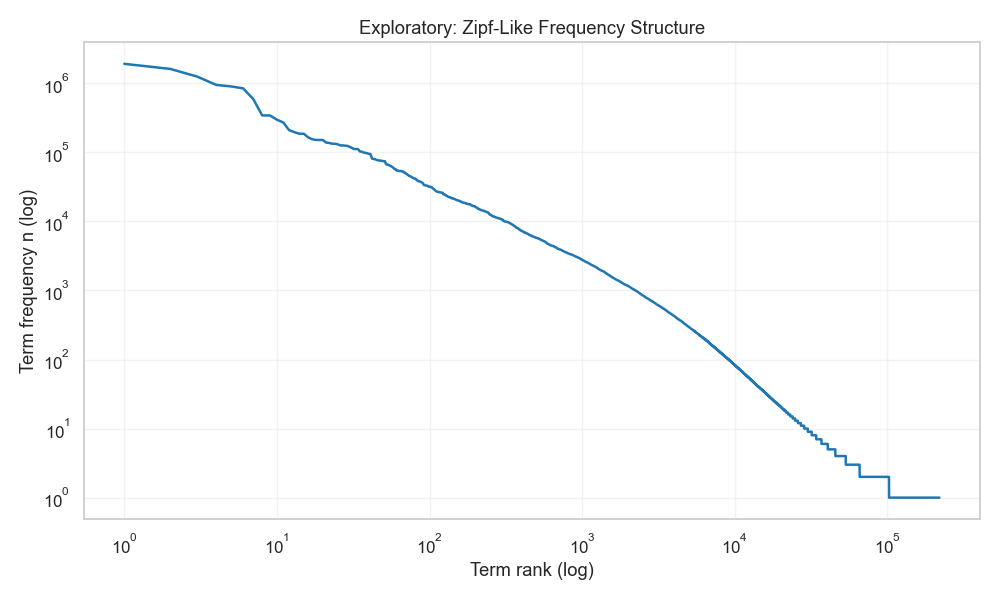
\includegraphics[width=\textwidth]{modern_explore_zipf.png}
\caption{Exploratory analysis: Zipf-like term frequency structure.}
\label{fig:explore_zipf}
\end{figure}

\begin{figure}[tb]
\centering
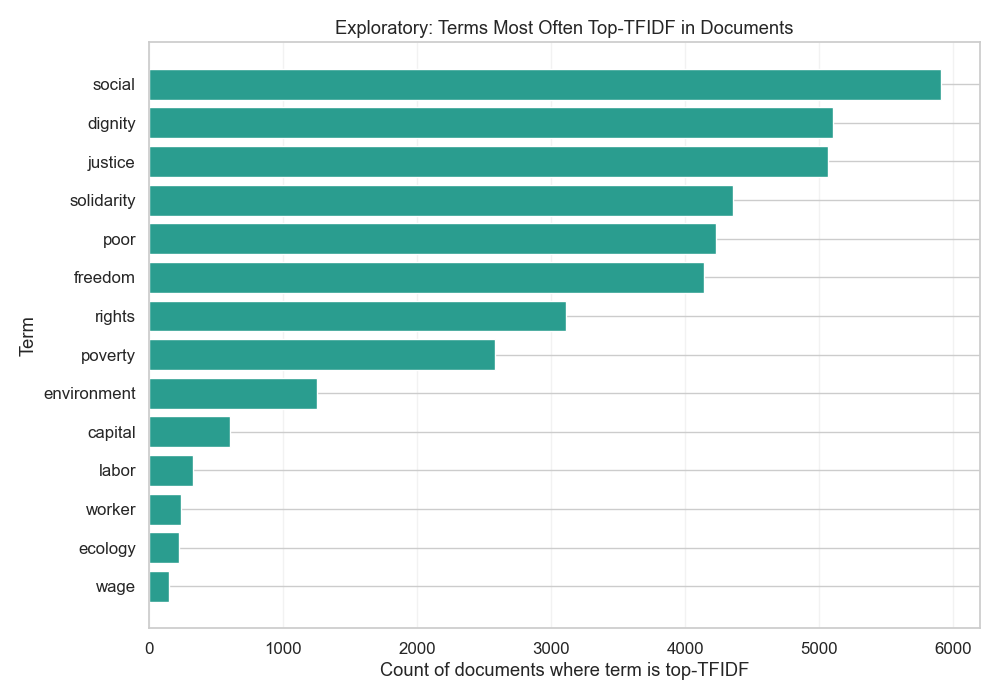
\includegraphics[width=\textwidth]{modern_explore_tfidf_salience.png}
\caption{Exploratory analysis: terms most often top-TFIDF across documents.}
\label{fig:explore_tfidf}
\end{figure}

\begin{figure}[tb]
\centering
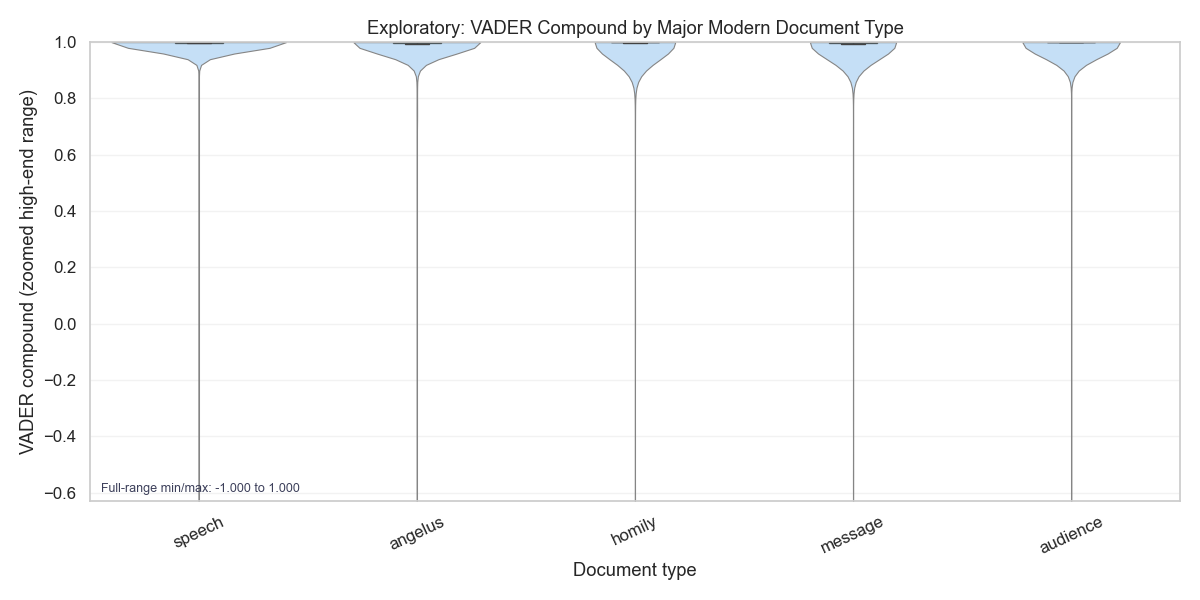
\includegraphics[width=\textwidth]{modern_explore_sentiment_types.png}
\caption{Exploratory analysis: sentiment distributions by major modern document type, shown with violin-plus-box summaries and a zoomed high-end axis (full min/max annotated in-plot).}
\label{fig:explore_sentiment}
\end{figure}

\begin{figure}[p]
\centering
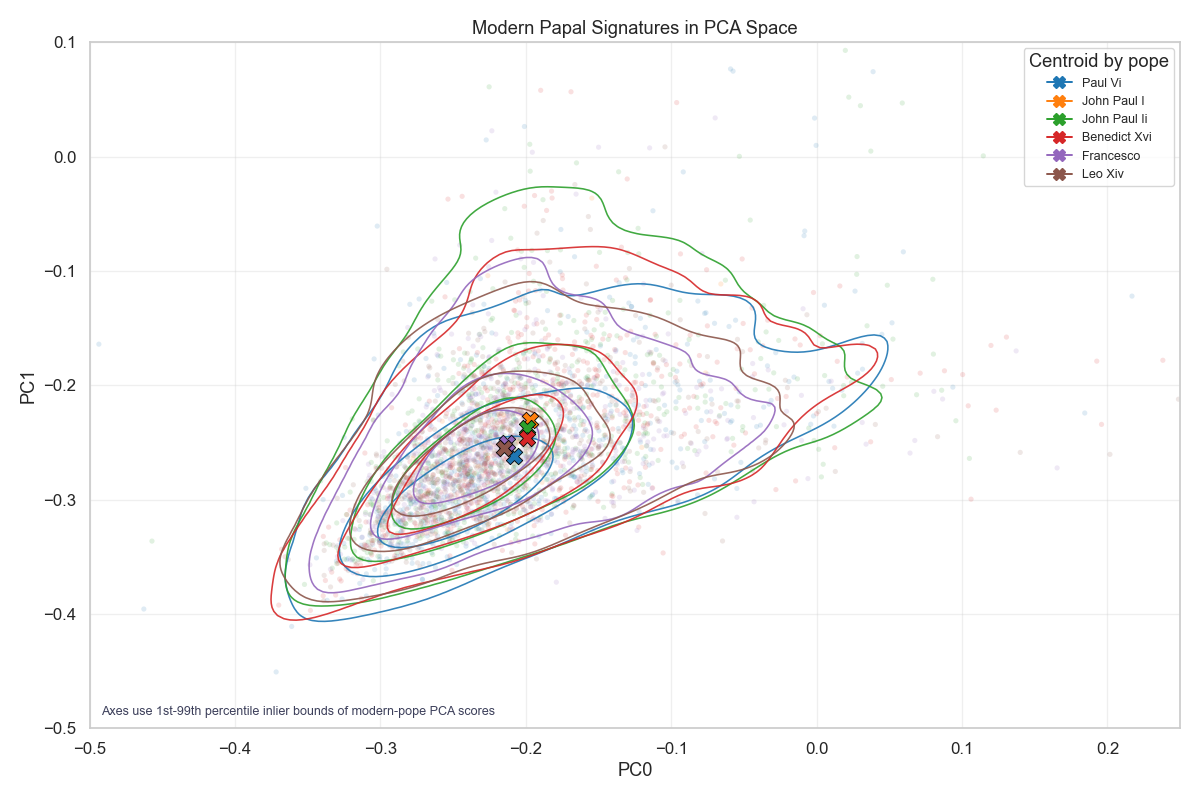
\includegraphics[width=\textwidth]{modern_rq1_pca.png}
\caption{RQ1: Modern papal signatures in PCA space with low-alpha samples, density contours, and centroid markers by pope.}
\end{figure}

\begin{figure}[p]
\centering
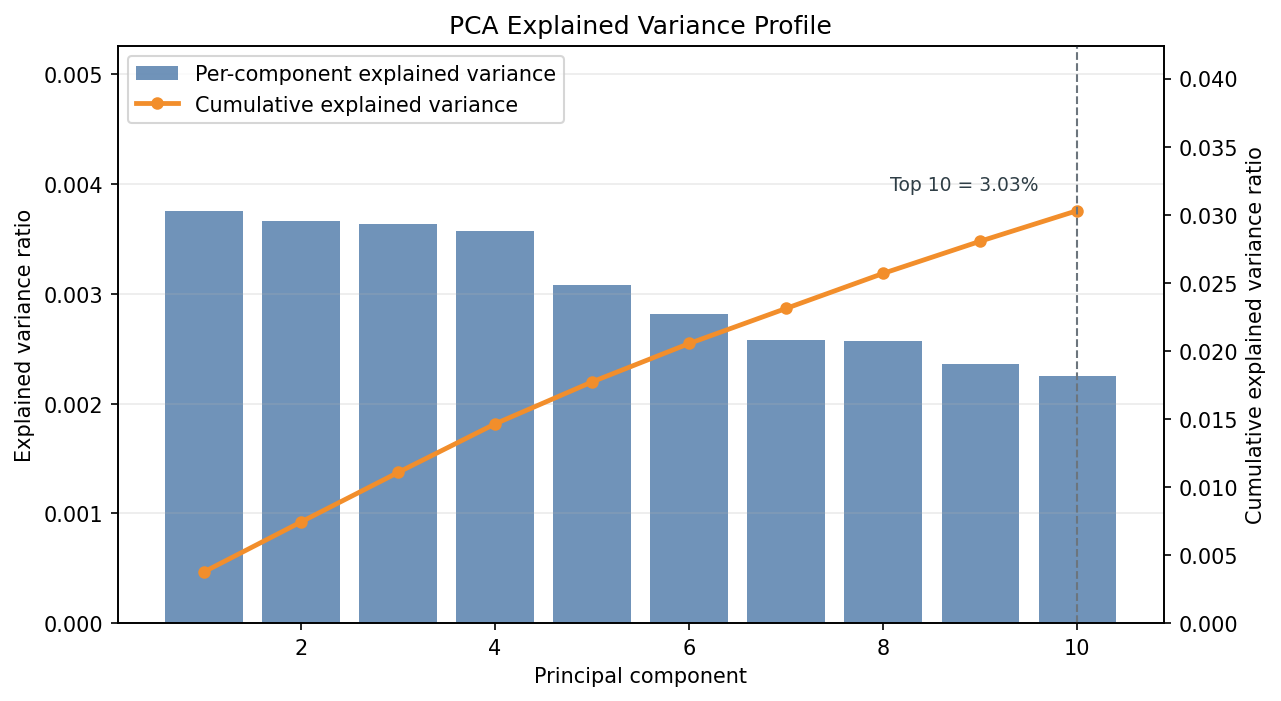
\includegraphics[width=\textwidth]{modern_pca_explained_variance.png}
\caption{PCA variance evidence: per-component explained variance and cumulative explained variance curve.}
\label{fig:pca_variance}
\end{figure}

\begin{figure}[p]
\centering
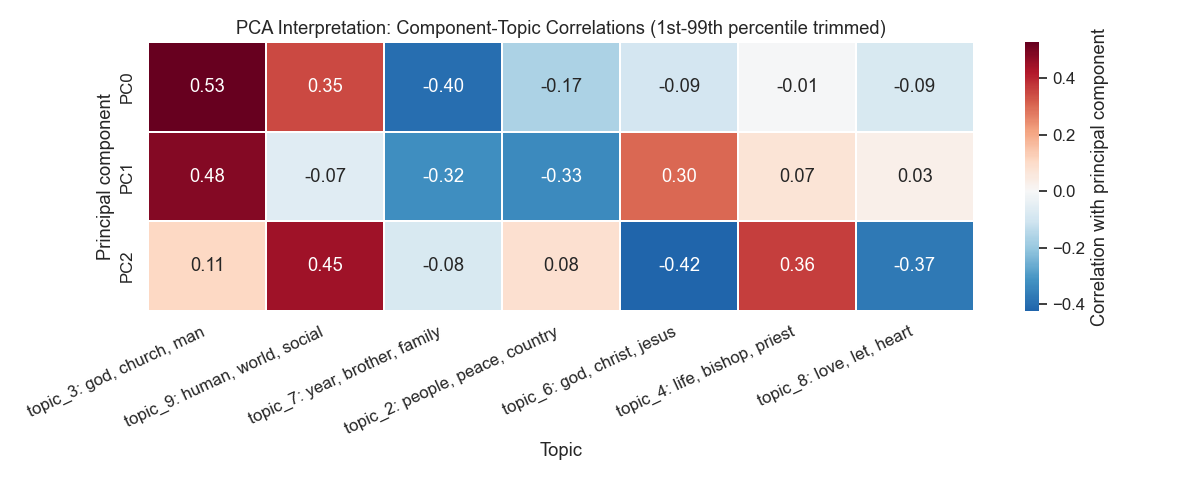
\includegraphics[width=\textwidth]{modern_pca_topic_corr.png}
\caption{PCA interpretation support: inlier-trimmed correlations between PC0--PC2 and referenced topics.}
\label{fig:pca_topic_corr}
\end{figure}

\begin{figure}[p]
\centering
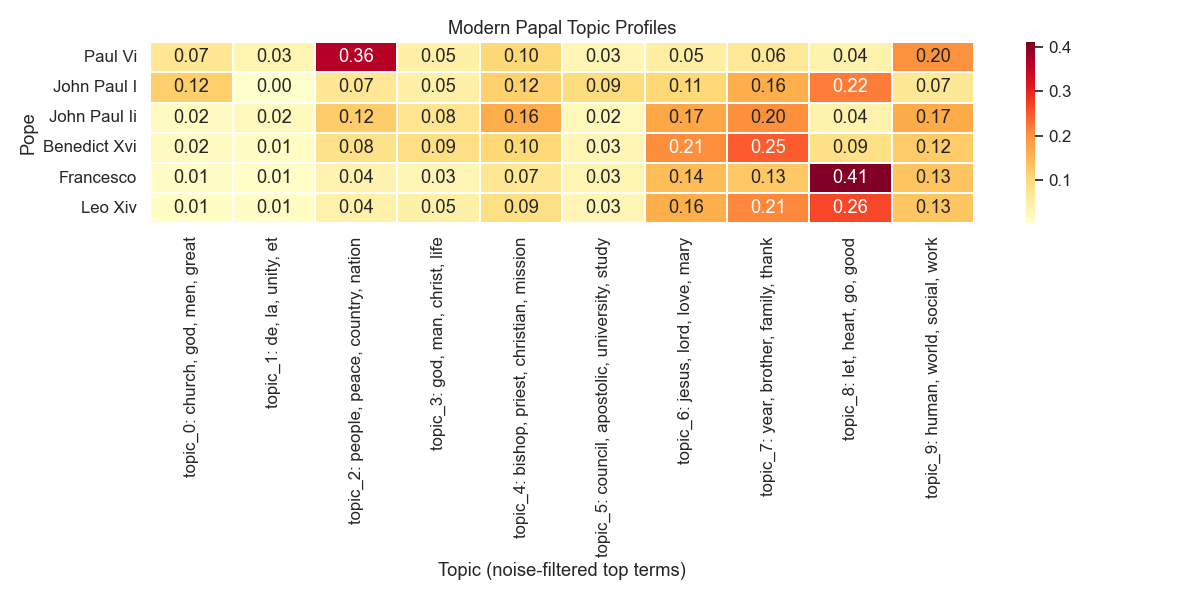
\includegraphics[width=\textwidth]{modern_rq1_topics.png}
\caption{RQ1: Mean modern topic weights by papacy, with noise-filtered semantic topic labels.}
\end{figure}

\begin{figure}[p]
\centering
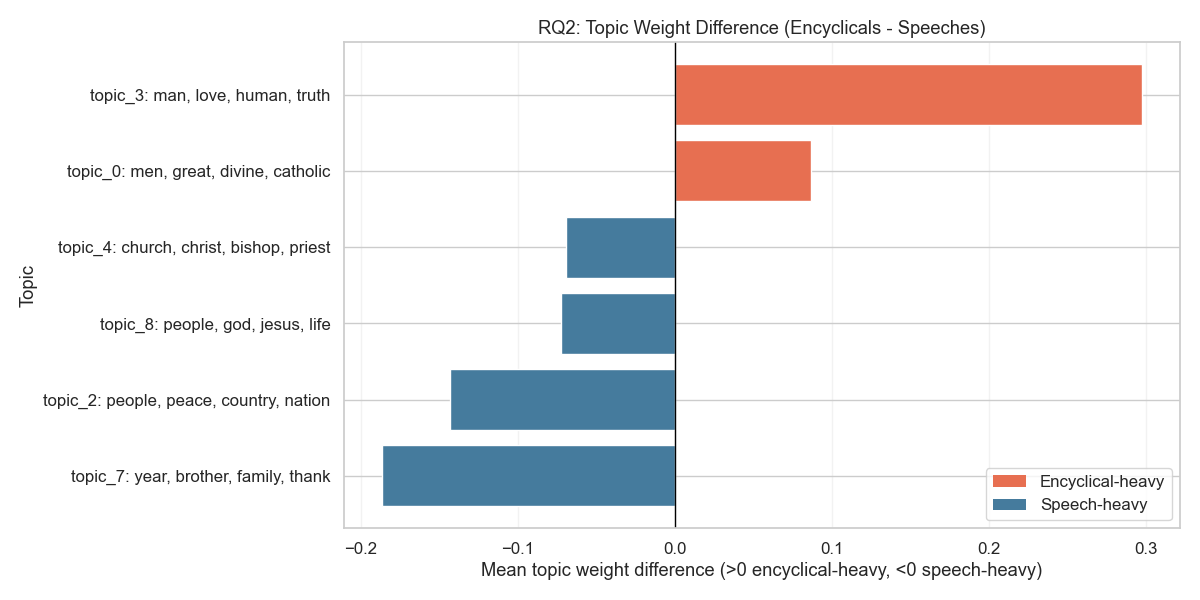
\includegraphics[width=\textwidth]{modern_rq2_encyclical_vs_speech_topics.png}
\caption{RQ2: Topic-weight deltas between modern encyclicals and speeches (encyclical minus speech), with explicit color legend for encyclical-heavy vs. speech-heavy topics.}
\label{fig:rq2_topic_delta}
\end{figure}

\begin{figure}[p]
\centering
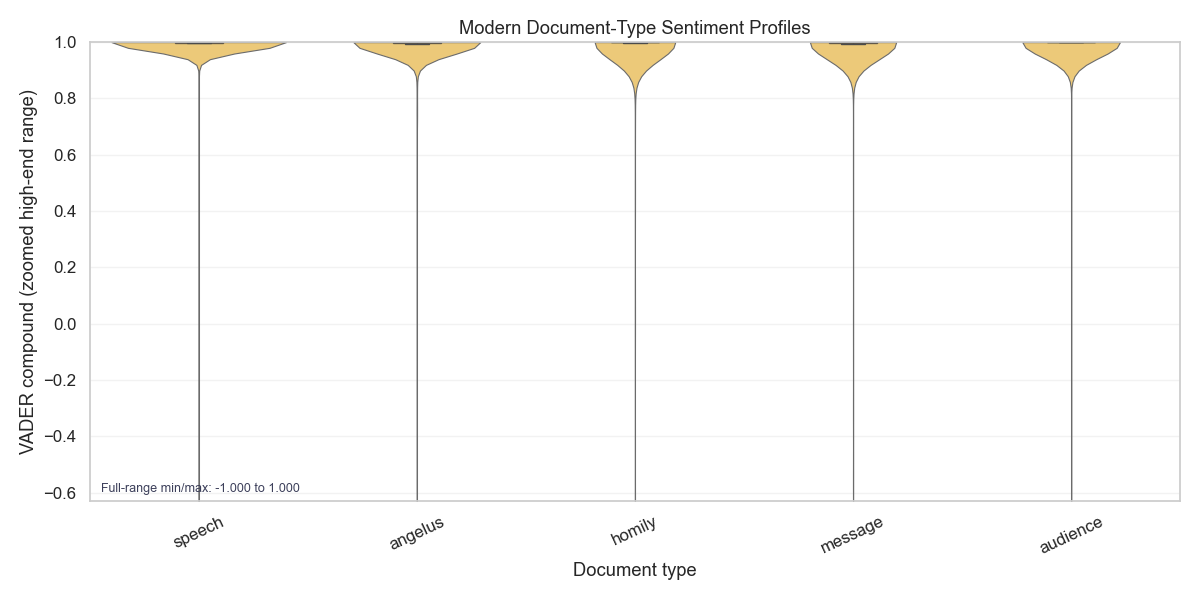
\includegraphics[width=\textwidth]{modern_rq2_doc_type_sentiment.png}
\caption{Supplementary RQ2 context: sentiment distributions by modern document type, using violin-plus-box summaries and zoomed high-end axis.}
\end{figure}

\begin{figure}[p]
\centering
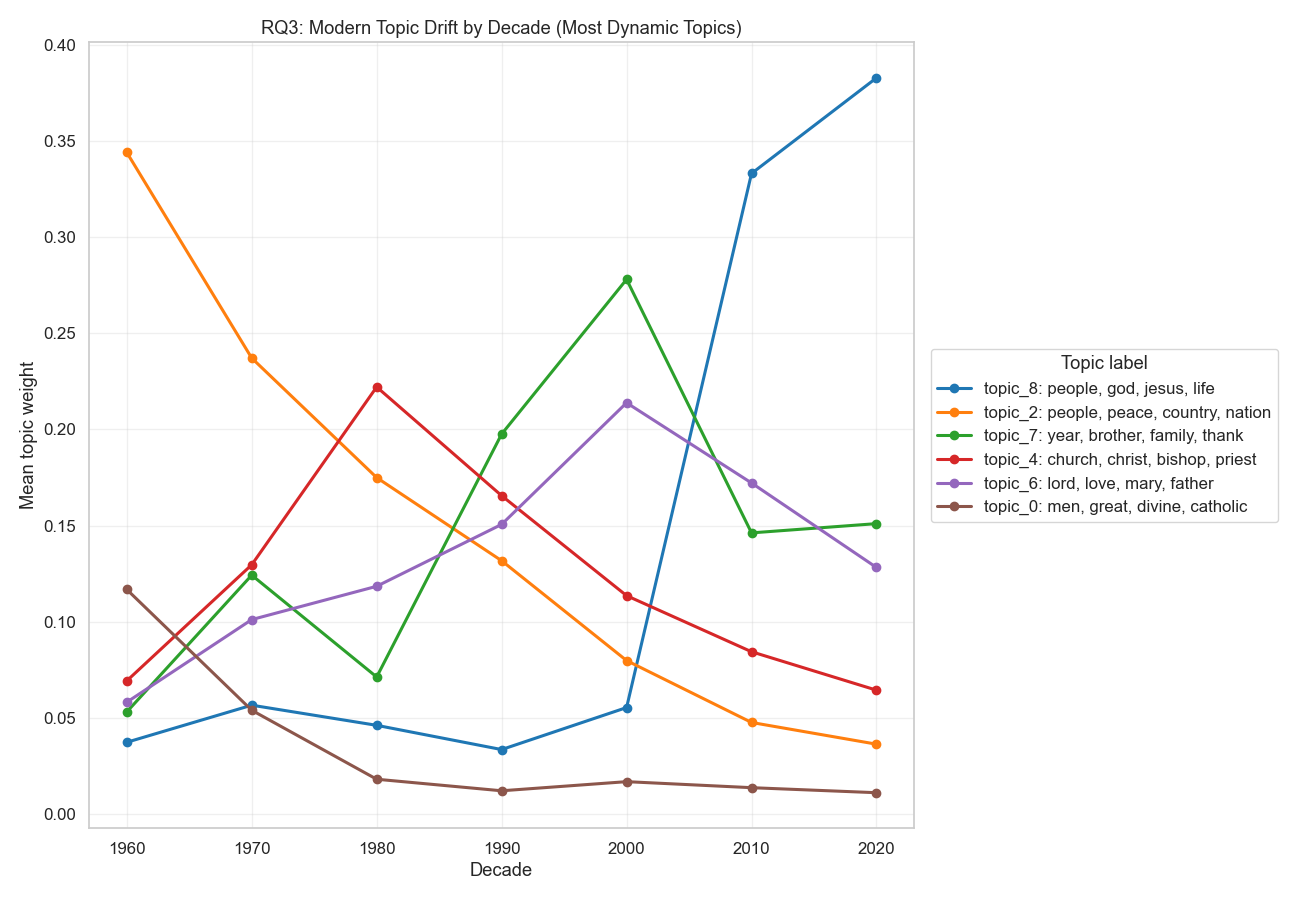
\includegraphics[width=\textwidth]{modern_rq3_topic_drift.png}
\caption{RQ3: Modern topic drift by decade for the most dynamic topics, shown as labeled trajectories in a single panel.}
\label{fig:rq3_topic_drift}
\end{figure}

\begin{figure}[p]
\centering
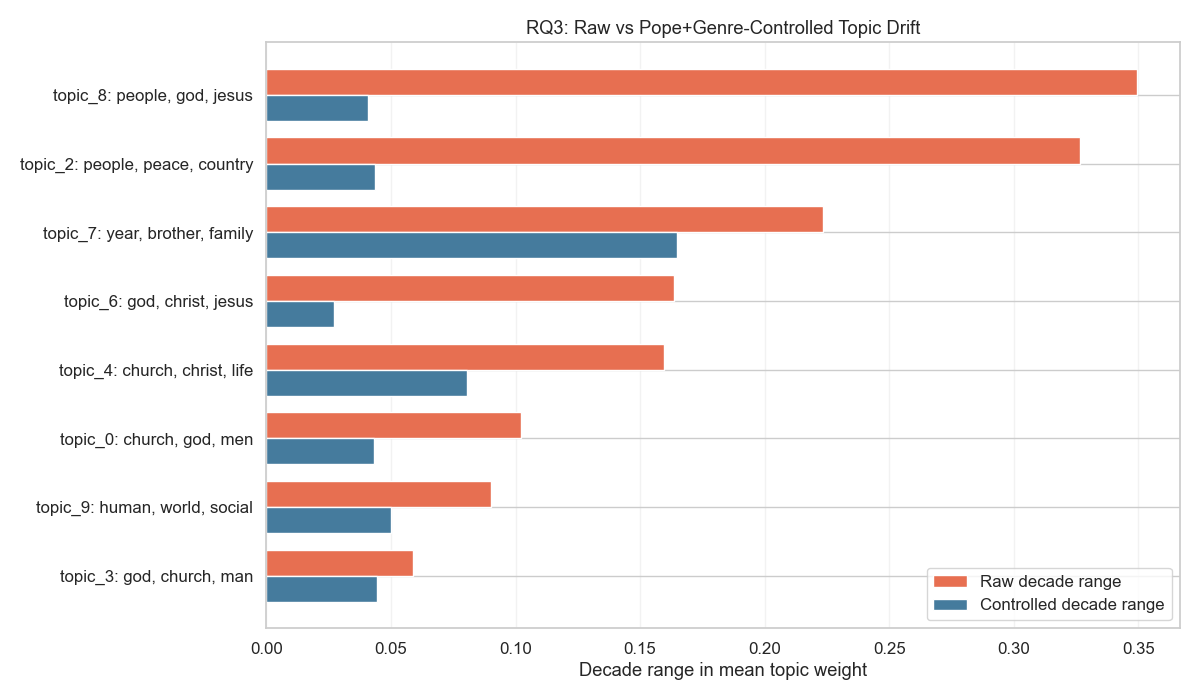
\includegraphics[width=\textwidth]{modern_rq3_raw_vs_control.png}
\caption{RQ3: Comparison of raw decade-range topic drift vs pope+document-type controlled decade-range drift.}
\label{fig:rq3_raw_control}
\end{figure}

\begin{figure}[p]
\centering
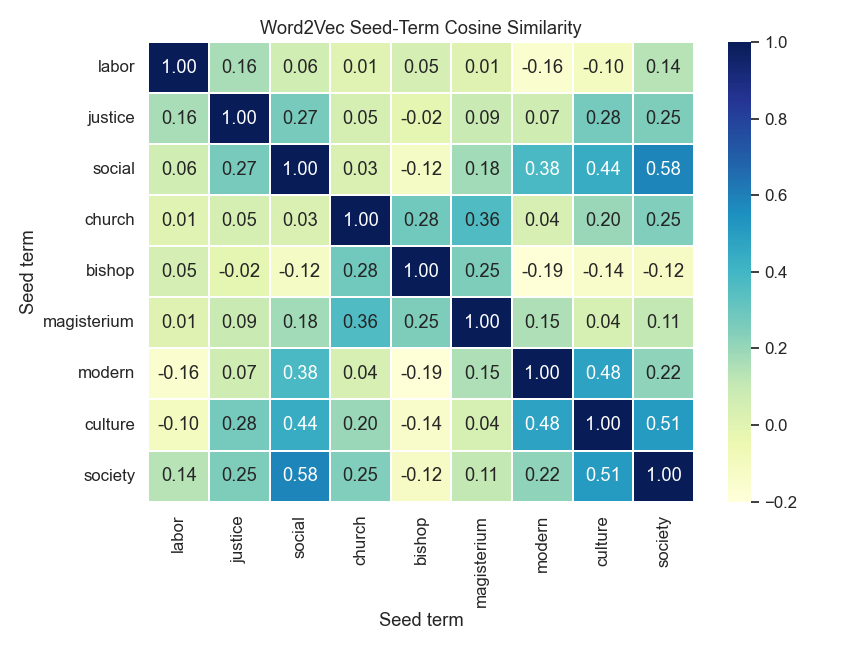
\includegraphics[width=\textwidth]{modern_w2v_seed_similarity.png}
\caption{Word2Vec evidence: cosine similarity among seed terms spanning doctrinal, social-ethical, and pastoral domains.}
\label{fig:w2v_seed_similarity}
\end{figure}

\end{document}
